\documentclass{article}
\usepackage[T1]{fontenc}
\usepackage[utf8]{inputenc}
\usepackage[margin=1in]{geometry}
\usepackage{fancyhdr} 
\usepackage{listings}
\usepackage[ruled,vlined]{algorithm2e}
\usepackage{amsthm}
\usepackage{amsfonts}
\usepackage{amssymb}
\usepackage{graphicx}
\usepackage[dvipsnames]{xcolor}
\usepackage{xy}
% \usepackage{url} % Commented out because hyperref provides similar functionality
\usepackage{parskip}
\usepackage{comment}
\usepackage{setspace}
\usepackage{enumerate}
\usepackage{multirow}
\usepackage{hyperref}
\usepackage{caption}
\usepackage{subcaption}
\usepackage{booktabs}
\usepackage{wrapfig}
\usepackage{times}

\captionsetup[figure]{font={small,it}}

\usepackage[backend=biber,style=numeric,sortcites,maxbibnames=99]{biblatex}
\addbibresource{references.bib}

\newcommand{\HRule}{\rule{\linewidth}{0.5mm}}
\newcommand{\Hrule}{\rule{\linewidth}{0.3mm}}
\newcommand{\classnum}{CS-GY 6313 B}

\makeatletter% since there's an at-sign (@) in the command name
\renewcommand{\@maketitle}{%
  \parindent=0pt% don't indent paragraphs in the title block
  \centering
  {\Large \bfseries\textsc{\@title}}
  \HRule\par%
  \textit{\@author \hfill \classnum}
  \par
}
\makeatother% resets the meaning of the at-sign (@)

\title{Assignment \#2: Misleading Visualization}

\author{Ivan Aristy}
% \classnum

\begin{document}
  \maketitle % prints the title block
  \thispagestyle{empty}
  % \vspace{-15pt}

References to papers and books look like this \cite{munzner2014visualization}. 

References to sections look like this: \autoref{sec:sec1}

References to figures look like this: \autoref{fig:fig1}

\begin{figure}[ht] % Change the position of your figure https://www.overleaf.com/learn/latex/Positioning_images_and_tables
    \centering
    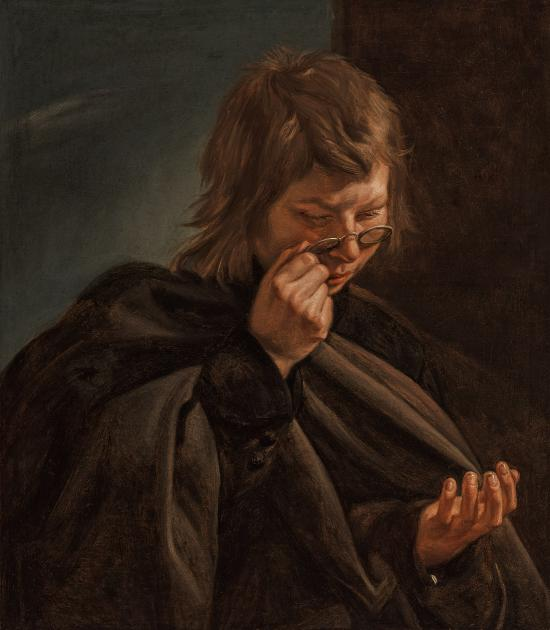
\includegraphics[width=0.75\textwidth]{figs/sight.jpg}
    \caption{
        Figure captions look like this. You can change the size of the figure using the \texttt{width} parameter in the \texttt{\textbackslash includegraphics} command. You can change the position of the figure using the position arguments in the \texttt{\textbackslash begin\{figure\}} environment command.
        URLs look like this: \url{https://www.mfa.org/exhibition/michaelina-wautier-and-the-five-senses}
    }
    \label{fig:fig1}
\end{figure}

\section{Visualizations}
\label{sec:sec1}

The following are the two Visualizations that I have created for this Assignment:

\begin{figure}[ht] 
  \centering
  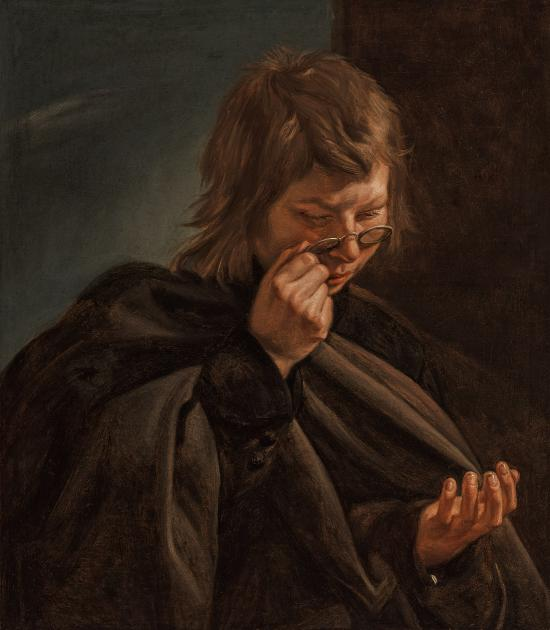
\includegraphics[width=0.75\textwidth]{figs/sight.jpg}
  \caption{
      Visualization \#1
  }
  \label{fig:Visualization1}
\end{figure}

% \begin{figure}[ht] 
%   \centering
%   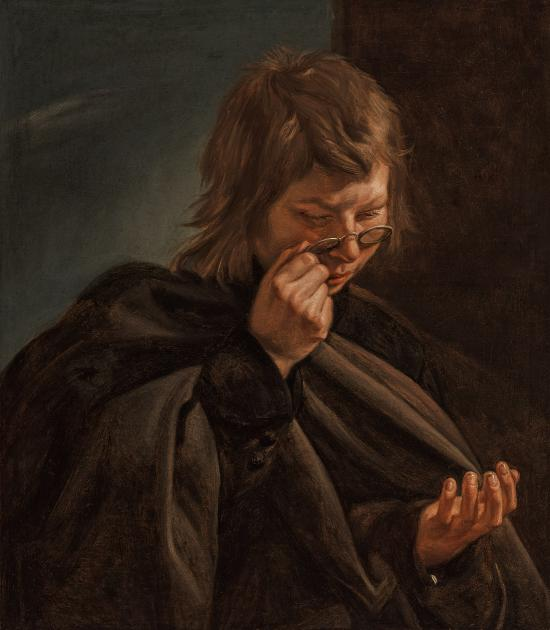
\includegraphics[width=0.75\textwidth]{figs/sight.jpg}
%   \caption{
%       Visualization \#2
%   }
%   \label{fig:Visualization2}
% \end{figure}

\section{}
\label{sec:sec2}

\subsection{Misleading Visualization}
\label{subsec:misleading}

\subsubsection{Topic Ideation}

For the Misleading visualization I had a few thoughts:

\begin{itemize}
  \item Immigration and Crime correlations: 
  Showing an extrapolated correlation between immigration and crime rates 
  could be made misleading by selecting data points that support a biased narrative.
  For example, not filtering by region, and actively sampling from regions with high crime rates.

  \item Ethnically Biased Drug Usage: 
  Using the "US Drug overdose death rates, by drug type, sex, age, race, and Hispanic origin" 
  \cite{drugOverdoseDeathRates} dataset, we use missleading bar charts to exaggerate the 
  correlation between hispanic heritage and drug consumption. Additionally, by 
  filtering out specific drugs we could make it especially

  \item Misleading use of colors to imply significance.
  \item Inappropriate use of 3D effects to distort perception.
  \item Cherry-picking data points to support a biased narrative.
\end{itemize}

\subsubsection{Topic Selection and Question}
\subsubsection{Misleading Qualities}


\newpage
\begin{refcontext}[sorting=nyt]
\printbibliography
\end{refcontext}

\end{document}

